\section{Materials and methods}
In this section I will describe the development of the interactive visualization
as well as the process of gathering information on how people use it.

\subsection{Helsinki region Travel Time Matrix}
Travel time matrix files,

\subsection{Requirements for the interactive map presentation}

% Why this must be considered
As mentioned earlier, cartographic visualization is often about tradeoffs.
The interactive map crafted here is no exception.
Rather, it is quite the opposite -- In addition to visual composition,  % TODO
many decisions must be made based on technical aspects. For example,
the sheer scale and detail of the dataset being visualized means that
instantaneous interaction with the map is not realistic
if no detail of the mapped data is to be sacrificed.
These kinds of tradeoffs are important to recognize,
since only through them is it possible to specify what
requirements should, or even could, be placed on the map application.

% Roughly what kind of a map? Why?
Based on the background study,
I made the decision to prioritize real-time interaction over minute detail in the map.
The goal of the map is to act as a dynamic overview to the entire travel time matrix,
and user interaction, whether it is 
This decision is what ultimately shapes the requirements for the mapped data,
and thus dictates what kind of processing should be done on the data.

% What interaction should there be in the map

% What requirements do the two above chapters place on the map

\subsection{Evaluation of data processing approaches}
In order to map the 


\subsection{Evaluation of serving approaches}
server approach

\subsection{Evaluation of web-mapping libraries}
mapping approach

Technical requirements for making the map happen:
\begin{enumerate}
	\item Preprocess the matrix to a mappable format
	\item A back-end to serve the matrix
	\item The web map application
\end{enumerate}

See figure \ref{fig:architechture} for an idea of the architecture.

\begin{figure}[H]
	\centering
	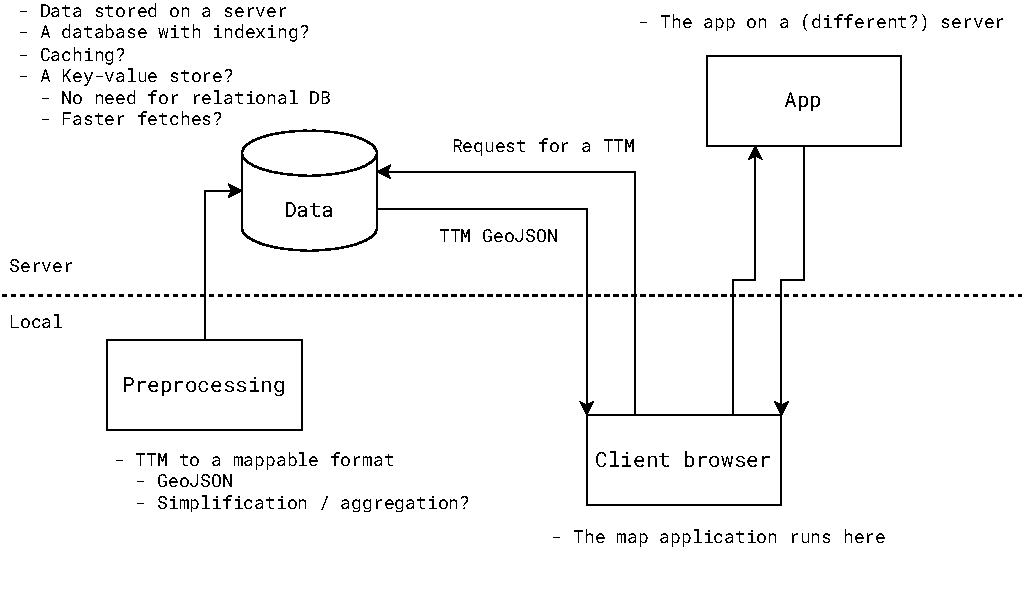
\includegraphics[width=1\textwidth]{images/architechture}
	\caption{Architecture}
	\label{fig:architechture}
\end{figure}

% I see the methods necessary to implement the visualisation belonging to two themes:
% Methods for figuring out how the map should be
% and methods for actually making the map be that way.

% For figuring out what the map should be like,
% I have (hopefully) at this point already formed some ideas from the background section.
% To complement those, and to keep the qualitative aspect of cartography relevant,
% interview(s) will be used alongside the development process.

% When developing the visualisation, the priority should be on the map application.
% However, the development must progress on all components as an iterative process,
% where producing a minimal working state should be the first goal.
% Something that, to some extent, works, makes discussion about the map possible,
% which in turn should keep development progressing towards the right direction.

% It should also be noted that the number of techical options for implementing the map is large.
% Questions such as which mapping library or UI framework to use,
% or how to preprocess the matrix data should be covered here too.
% Depending on the need and extent of comparisons between different technologies,
% some synthesis could be formed about that too.

\subsection{Survey design}
structure of the survey,
analysis of the survey data.
